% !TeX root = ../Thesis.tex
\chapter{Fundamentals}\label{chap:fundamentals}
This chapter provides necessary fundamentals for the subsequent thesis.
First, the HippoCampus \ac{uauv} is presented as an example of an underactuated small-scale underwater robot.
This is followed by throughout review of motion planning methods for submerged robots.
Notably, this review also considers non-marine domains such as the aerial domain, as research in these areas is expected to provide helpful insights into promising motion planning strategies, particularly agile planning.

\section{HippoCampus $\mu$AUV Platform}\label{sec:hippo-platform}

The HippoCampus \ac{uauv} is an agile underwater robot developed at the Institute for Mechanics and Ocean Engineering. It is a representative of the recently evolved class of underwater vehicles called hydrobatic \cite{hydrobatic}. In this chapter, an overview of the hard- and software architecture is given.

\subsection{Hardware}
The iteration of the HippoCampus \ac{uauv} designed for this thesis is depicted in \Cref{fig:new-vehicle-design} is \unit[30]{cm} in length and \unit[8]{cm} in diameter.
\begin{figure}[h!]
    \centering
    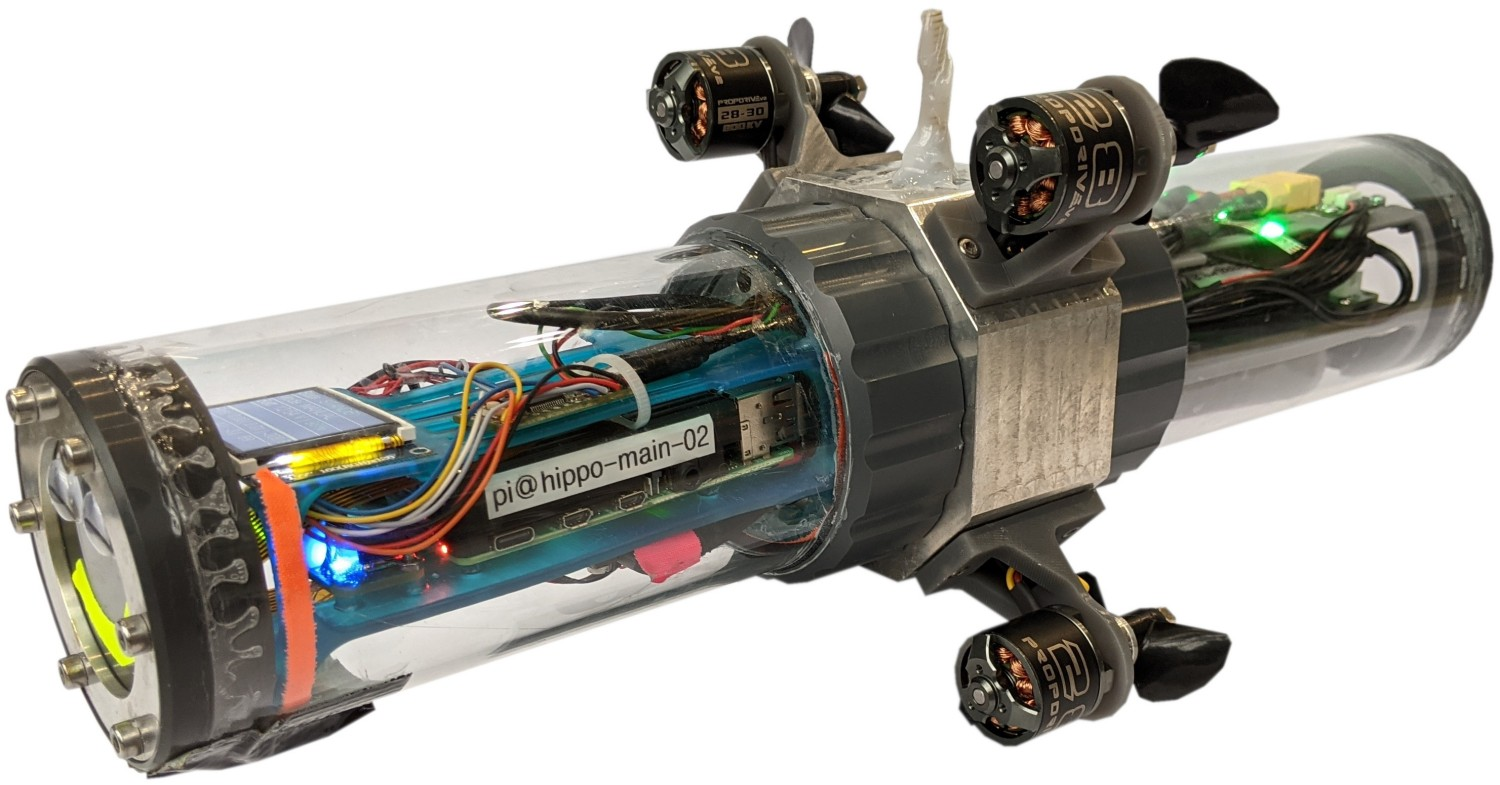
\includegraphics[width=0.4\textwidth]{hippo_picture}
    \quad\quad
    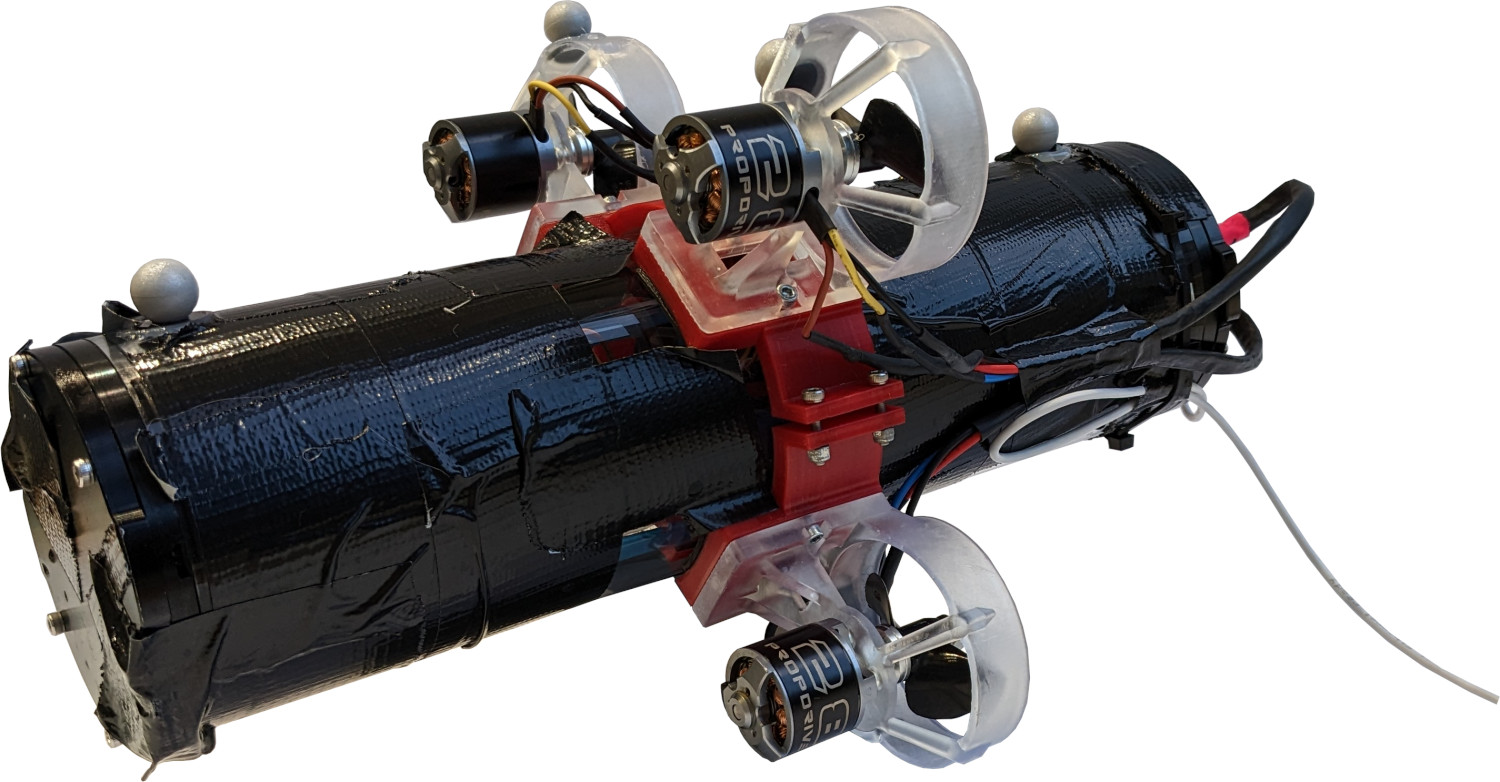
\includegraphics[width=0.4\textwidth]{hippo3_picture}
    \caption{HippoCampus $\mu$AUV in its heavy configuration (\textit{left}) and redesigned version based on BlueRobotics off-the-shelf components (\textit{right}).}
    \label{fig:new-vehicle-design}
\end{figure}
In contrast to its predecessors, this version is built from off-the shelf components, with the sole exception of the 3D-printed mounts for the electric components and motors. 
Its mass sums up to \unit[2.31]{kg} including additional ballast mass of approximately \unit[150]{g} to neutralize buoyancy.

Essential hardware components are the four thrusters, the \ac{fcu} and the onboard computer. The thruster configuration resembles those of quadcopters. The \textit{X}-configuration enables direct actuation of forward thrust and all three rotational degrees of freedom. Hence, HippoCampus is an underactuated but still highly agile underwater robot, due to its small size and low weight.

The \ac{fcu} is a PixRacer, that is used as flight controller \acp{auv}. It features an \ac{imu}, including an accelerometer, gyroscope, and magnetometer which are used for onboard state estimation. Low-level control loops are usually executed on the \ac{fcu}. High-level controls and mission planning tasks, as well as computational heavy operations such as image processing, are the responsibility of the onboard computer. The onboard computer is a Raspberry\,Pi 4B with an ARM\,A72 quad-core processor.

\subsection{Software Architecture}
The general software architecture of the HippoCampus platform is shown in \Cref{fig:software-architecture-overview}. 
For a detailed description the reader may refer to \cite{duecker-phd}. 
\begin{figure}
	\centering
     \def\svgwidth{12cm}  
	\input{images/02/03_hippo_system_architecture_draft.pdf_tex}
	\caption{System architecture of the HippoCampus $\mu$AUV \cite{duecker-phd}.}
    \label{fig:software-architecture-overview}
\end{figure}
The modular design is divided into modules assigned to the \ac{fcu} and modules assigned to the onboard computer.
Two different frameworks are deployed, PX4 \cite{PX4} and \ac{ros} \cite{ros}.
Both are similar from the perspective that both frameworks implement a publish-subscribe pattern.
The interconnection between PX4's \ac{uorb} running on the \ac{fcu} and \ac{ros} on the onboard computer is realized via a combination of \ac{mavlink} \cite{mavlink} and MAVROS.
Since \ac{uorb} is restricted to intra-process communication, communication with external devices is done via \ac{mavlink}.
\ac{mavlink} is a communication protocol for \acp{uav}.
The interface between \ac{mavlink} and \ac{ros} is MAVROS. It is a bidirectional bridge, translating messages from \ac{mavlink} to corresponding \acs{ros}-messages and vice versa. This whole setup is depicted in \Cref{fig:ros-px4-communication}.
\begin{figure}
	\centering
	\includesvg[width=0.9\textwidth]{images/02/software_architecture_old}
	\caption{HippoCampus software architecture with multiple layers of abstraction. Communication between \acs{ros} (left) and PX4 (right) via \acs{mavlink}. On the \acs{ros}-side this requires the MAVROS package, while on the PX4-side, the \acs{mavlink} transceiver package is used.}
    \label{fig:ros-px4-communication}
\end{figure}


\subsubsection{Limitations of the current software setup}\label{sec:sw_limitatations}

There are several limitations and drawbacks regarding the status quo of the HippoCampus software architecture depicted in \Cref{fig:ros-px4-communication}.
It is clear that the communication between the onboard computer and the \ac{fcu} involves several layers of abstraction on multiple conversions of messages.
This renders the communication between the onbaord computer and the \ac{fcu} more complex and less efficient.
Furthermore, \ac{ros} was not designed with real-time capabilities, support for embedded systems, or unreliable communication channels in mind \cite{ros2}. Finally, the final \ac{ros} distribution is reaching its end-of-life in May 2025.

%


\section{Review on Motion Planning}
\label{sec:review-motion-planning}
We refer to motion planning as either path planning or trajectory planning. Path planning only considers the spatial aspect of motion, while for trajectories there is a relation between the geometric path and time. 
For many applications, it is convenient to decouple the path planning aspect from the temporal planning. 
However, by assigning a velocity profile to the planned path, a trajectory can be obtained after the path planning problem is solved. Hence, no rigorous distinction between trajectory and path planning is made in the course of this section.
The findings of this review are summarized in \Cref{tab:state_of_the_art}.

\subsection{Underwater Motion Planning}
\label{sec:underwater-motion-planning}

In the following, a selection of widely used algorithms for solving underwater path planning problems is introduced, their concept briefly summarized and example applications in the domain of \acp{auv} are presented. This aims to provide a sufficient overview of the state of the art, to point out strengths and limitations of existing underwater path planning methods.

\cite{Panda20} presents a comprehensive overview of various path planning approaches for single- or multi-\acsp{auv} scenarios. Since multi-agent systems are not the focus of this thesis, the interested reader may refer to \cite{Panda20} for more information on this topic.

%  \cite{Gomez15} classifies different path planning methods: geometric methods, graph- and tree-based methods and artificial potential fields methods. For this thesis, the categorization by the useare d techniques seems less useful than grouping the methods by their field of application.

\subsubsection{Graph- and tree-based Methods}
According to \cite{Gomez15}, methods falling in this category attracted the strong attention of researchers in recent years. 
A lot of well-known and often-used algorithms belong to this group of path planning methods, such as A*, \ac{rrt}, or \ac{fmm}.


\paragraph{Grid-based Search}
For grid-based approaches like A*, the vehicle states or the environment are discretized and encoded as nodes in a graph, building the search space. Costs are assigned to the edges connecting the nodes. Depending on the used algorithm, a path is searched that connects the initial state with a desired goal state.
To obtain, for example, the shortest path, the costs can be defined as the euclidean distance between discrete positions in the environment. The nodes of the graph encode the discretized environment.
Subsequently, a search algorithm guaranteeing optimality can be deployed to find the path with the lowest costs, if one exists. Due to dicretization, accuracy naturally decreases. A smaller grid size counteracts this problem, but increases the search space and therefore the computational costs for finding a solution.

The authors in \cite{Fernandes2015TowardsAO} declare A* in its generic form as generally not suitable for mobile robots with time constraints, due to the performance costs associated with traversing the state space if replanning is required. Still, there exist various publications applying variants of A* in the context of path planning for mobile robots and \acp{auv} in particular.

Applications of A* in the domain of \acp{auv} can be traced back to the 1990s \cite{Carroll92}, while still being extended in recent works \cite{zhang20}. Common to these approaches is the application for oceanic environments, where obstacles are assumed to be static, traveled distances to be large, and vehicle dynamics not to be relevant. The main focus often lies on considering ocean currents for path planning.

Another algorithm used for grid-based search is \ac{fmm}. The principle of \acs{fmm}-based path planning is based on simulated wave propagation in order to obtain distance fields. The procedure is depicted in \Cref{fig:fmm}
\begin{figure}
    \centering
    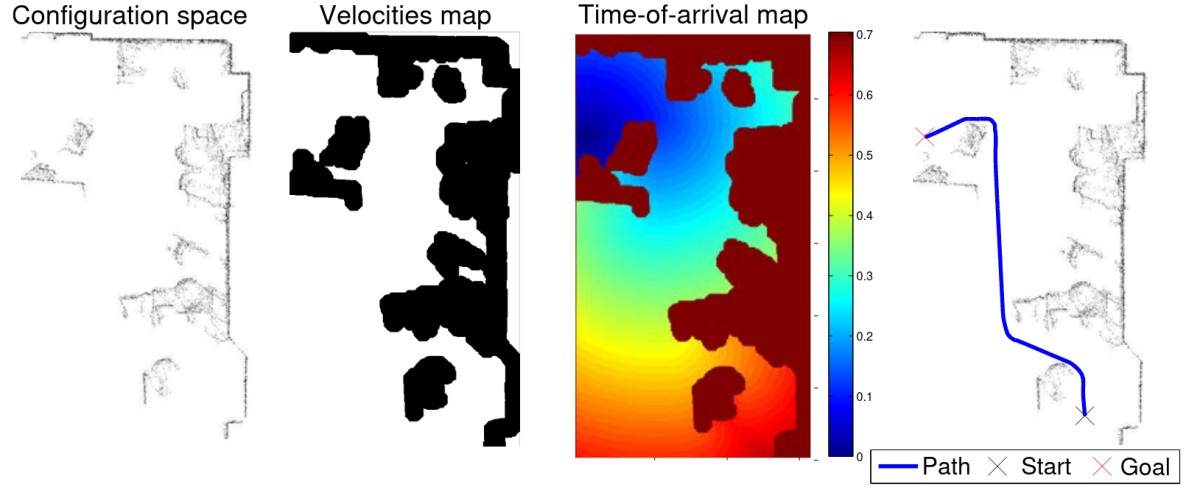
\includegraphics[width=0.8\textwidth]{images/02/fmm}
    \caption{Visualization of path planning with \ac{fmm} \cite{Gomez15}.}
    \label{fig:fmm}
\end{figure}
Obstacles in the environment can be taken into account and in the case of well-known propagation, the optimal path between the start and goal position in terms of distance can be found. Modifications to the wave propagation can be used to compute paths for different requirements.

The authors in \cite{Petres09} present a modification of \ac{fmm} called \acs{fmm}*. They exploit the reduced computation due to an appropriate heuristic function to solve path planning problems in dynamic environments, for instance when the environment changes or is partially unknown. The authors observe improved performance regarding computation time compared to A*. Additionally, they were able to enforce environment constraints for the planned path.

\paragraph{Sampling-based Search}

A typical representative of sampling-based methods is \ac{rrt}. Even though the original version of \ac{rrt} does not provide optimality guarantees, it compensates for that by being able to efficiently solve complex planning problems, that are possibly high-dimensional \cite{Devaurs16}. Randomly sampled points are connected to generate a tree to find a path between initial and goal state.

In \cite{Young13}, the authors present a path planning approach based on \ac{rrt} for \acp{auv} in the presence of obstacles. Kinematic constraints, such that the vehicle can only move with certain velocity limits, are respected. A model for the hydrodynamic properties of the vehicle is not considered, though.

The problem of non-optimality is addressed in \cite{Karaman11} with a modification of \ac{rrt}, called anytime \ac{rrt}, though not applied in the underwater domain. The idea is to find a solution as fast as possible and improve the solution if given further computation time. This renders the approach especially useful for dynamic environments.

An informed variant of \ac{rrt}, called RRT*, is used in \cite{Ma18} for terrain-aided navigation for long-range navigation of \acp{auv}.

\subsubsection{Artifical Potential Fields}
The basic idea of this path planning approach is to model the robot as electric charge \cite{Gomez15}. Obstacles are represented by charges with the same sign. Hence, the robot is repelled from obstacles. The goal state is modeled as a charge with an opposite sign and therefore attracts the robot. To find a way to the goal, the path minimizing the energy of the robot is searched, which can be accomplished by following the steepest gradient. The main drawback of this method is that it is not guaranteed that the robot is not trapped inside a local minimum. 

An improvement over the basic method of potential fields in the context of path planning for \acp{auv} is presented in \cite{Fu-guang05}. The authors suggest a heuristic to escape the local minimum in the vicinity of concave obstacles.

\subsubsection{Model Predictive Control}

Though actually a \textit{control} and not a path planning method, \ac{mpc} can still be used for path planning problems, as will be presented below. In \ac{mpc} methods the future state of a robot is predicted, based on a dynamic model of the robot. The future states depend on system inputs. By defining a cost function, an optimal solution regarding the control inputs to reach a desired state can be computed. To close the feedback loop, this optimization is performed at every time step. Hence, external disturbances and model inaccuracies are considered. But this also constitutes one of the major disadvantages of this method, as the computation of the optimal solution in each time step is usually computationally expensive.

\ac{mpc} in the area of path tracking for \acp{auv} has been presented in \cite{Shen16}. The authors use a multi-objective model predictive control framework and prove the validity of their approach in a simulation of the Saab SeaEye Falcon. In \cite{Heshmati18}, a waypoint-tracking controller, implemented as nonlinear \ac{mpc}, is proposed. The presented control scheme considers ocean currents, thruster saturation, and velocity limits and incorporates obstacle avoidance. The latter proves this approach to be promising for low-level maneuvering. The waypoints can be provided by a high-level mission planner and the model predictive controller is responsible for reaching them without violating the constraints.



\subsection{Review on Agile Path Planning Methods}
In this section, a brief review on agile path planning methods is given. As the previous section on path planning for \acp{auv} indicated, the problem of \emph{agile} path planning is underrepresented in the literature. Hence, in this section, the review is extended to the aerial domain. Due to the similarity in the design of small-scale \acp{uav} and \acp{uauv}, it is likely that findings in the aerial domain can be transferred to the area of hydrobatic \acp{uauv}.

In \cite{MellingerKumar11} the authors present a minimum snap trajectory generation method for quadrocopters. This approach is demonstrated to be real-time capable. The trajectory is defined by \emph{keyframes}, i.e. a position and a yaw angle, and corridor constraints between keyframes, as seen in \Cref{fig:mellinger}.
\begin{figure}
    \centering
    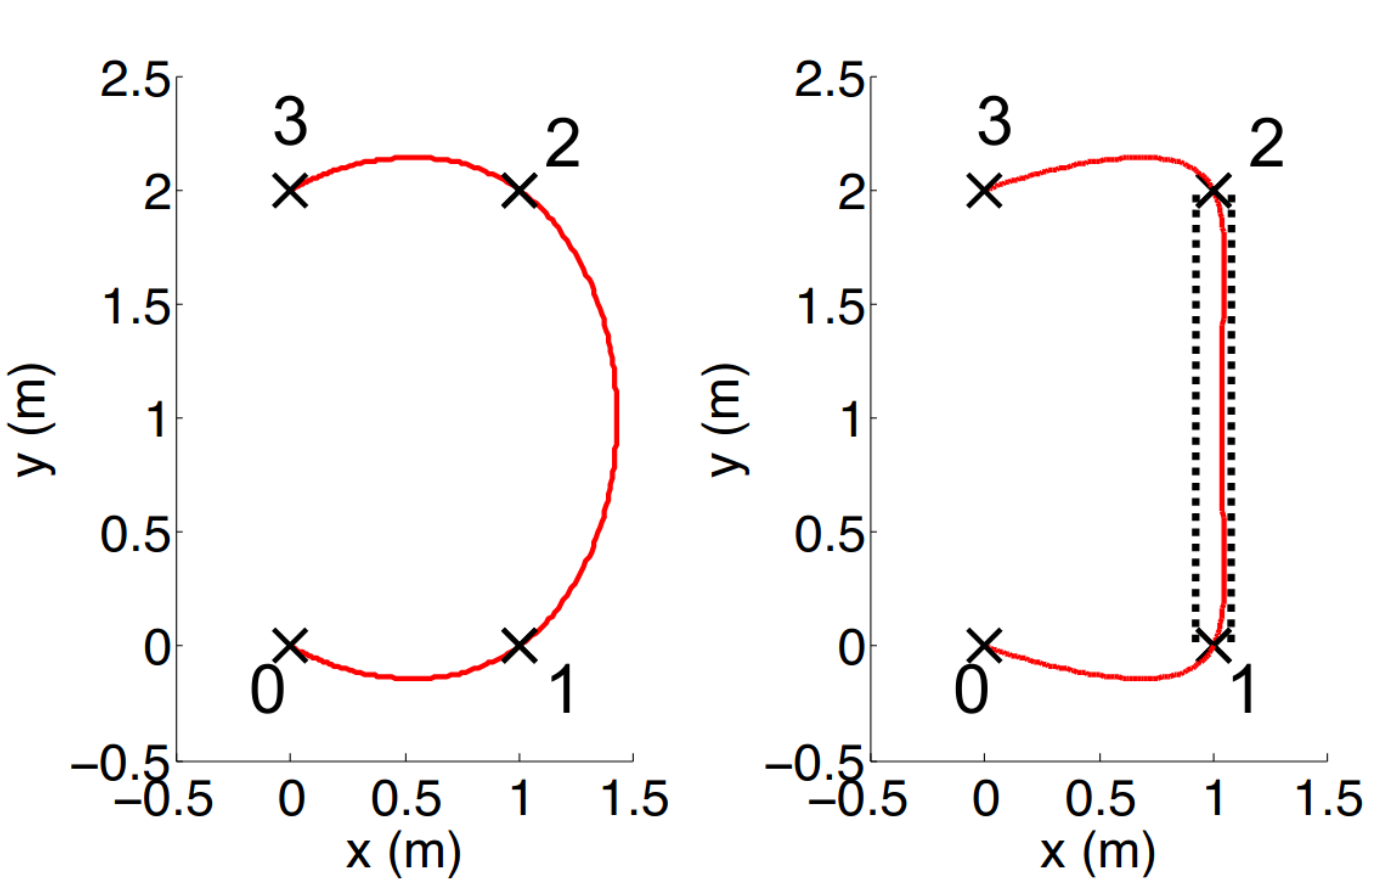
\includegraphics[width=0.6\textwidth]{images/02/mellinger.png}
    \caption{$xy$-plot of a minimum snap trajectory with keyframes depicted as crosses. On the left the trajectory has no corridor constraints, on the right, the corridor constraint is visualized as a dotted rectangle \cite{MellingerKumar11}.}
    \label{fig:mellinger}
\end{figure}
The corridor constraints can be used to navigate the vehicle through narrow gaps. General obstacle avoidance is not possible with this method, though.
The capability of this approach is demonstrated in experiments, where the quadcopter was able to fly through a thrown circular hoop, reaching velocities of \unit[3.6]{m/s}.

The authors in \cite{Hehn11} propose a trajectory generation framework for minimal-time trajectories. They consider the dynamic model of the \ac{uav} and solve for the optimal trajectory for each degree of freedom separately, by decoupling the translational degrees of freedom. The trajectory generation system is used in a closed-loop control scheme similar to \ac{mpc}. The authors face challenges with respect to the tracking performance when decelerating quickly from high velocities, caused by aerodynamic effects. They highlight the advantage of computational efficiency.

A combination of minimum snap trajectories and \ac{rrt} is presented in \cite{Richter16} and \cite{Shi20}.
\ac{rrt} is used as a high-level planner whereas the minimum snap trajectory generator is used to compute smooth trajectories suitable for the dynamics of \acp{uav}. 
The authors address the challenges of indoor navigation and use \ac{rrt} to generate waypoints as piece-wise linear paths to reach a goal position in presence of a cluttered environment. Subsequently, the waypoints are connected smoothly by minimum jerk trajectories.
The proposed implementation sacrifices the asymptotic optimality of \ac{rrt}* in favor of dynamically more suitable paths and reduced computation time. Even though the computation time could be reduced by a factor of 40, the computation time remains in the order of several seconds. Hence, the approach is not capable of accounting for dynamic obstacles.

In \cite{Mueller13}, a state-to-state trajectory generation method for quadrocopters is presented. The focus lies on the computational efficiency of the algorithms.
Instead of regarding the constraints during the trajectory planning phase, thousands of trajectories are generated based on appropriately chosen target states.
Afterward, their feasibility with respect to the vehicle dynamics is verified.
Based on this, all trajectories resulting in infeasible solutions are discarded.
This way, the computation time can be considerably reduced in comparison to other methods.
The authors suggest using the trajectory generation system in a control scheme resembling \ac{mpc} and similar to \cite{Hehn11}, i.\,e. the trajectories are recomputed in each control step and the first input of the selected trajectory is used as the input command. 
The trajectories are polynomials of order five and are optimal regarding jerk.
The authors demonstrate the performance of their approach in the scenario of a quadcopter equipped with a racket to hit a ball toward a target. The same algorithm is used in \cite{MuellerHehn15} applied to the problem of catching a thrown ball and extended in \cite{Bucki19} by an obstacle avoidance method, handling dynamic convex obstacles.


\subsection{Discussion}



We observe that the problem of path planning for \acp{auv} has usually been examined for traditional \acp{auv}, operating in ocean environments.
Hence, the publications often focus on problem characteristics relevant to the marine domain.
For instance, ocean currents are considered of higher priority than accounting for vehicle dynamics.
Since traditional \acp{auv} are very heavy and slow in relation to their size, it is questionable whether path planning approaches for this type of vehicles would be directly transferable to the domain of hydrobatic \acp{uauv}, agreeing with \cite{hydrobatic}.

Furthermore, many approaches solve the problem for static environments, as it is usually assumed when deploying A*-based concepts. This is reasonable if mainly the geometric restrictions caused by the coastal line and constant ocean currents are of concern. As a consequence, these algorithms cope with dynamic changes and re-planning rather badly. Moreover, larger \acp{auv} have usually more computational power and are less restricted with regard to the computational demands of the employed algorithms.

Hence, it seems more promising to consider the agile trajectory planning and tracking proposes published for \acp{uav} and benefit from the research progress made in the past years in the fields of aerobatic and agile maneuvering. The methods in \cite{Mueller13,MuellerHehn15,Bucki19} are promising to push the progress regarding agile maneuvering of \acp{uauv}, when successfully transferred to the underwater domain. Consequently, the methods presented in this thesis are based on the methods of the mentioned publications.


\begin{landscape}
\begin{table}[p]
\renewcommand{\arraystretch}{1.0}
    \caption{Overview on (agile) path planning methods.}
		\hspace*{-1.5cm}  % move table down (left in landscape) - tabular width: 
		\centering
		% change column width: >{\hsize=1.5\hsize\linewidth=\hsize}
		% >{\hsize=0.5\hsize\linewidth=\hsize}
		\begin{NiceTabular}
            {
            %%%%% Leider scheint die beste Methode wirklich hardgecodete Spaltenbreiten zu sein - hier am Ende rumspielen
            >{\centering\scriptsize\arraybackslash}m{3.5cm} % Example
            >{\scriptsize\centering\arraybackslash}m{1.1cm} % Domain
            >{\centering\scriptsize\arraybackslash}m{2cm}   % Method
            >{\centering\scriptsize\arraybackslash}m{3cm}   % Optimality
            >{\centering\scriptsize\arraybackslash}m{1.5cm}   % Obstacles
            >{\centering\scriptsize\arraybackslash}m{8.8cm}   % Comments
            }
            \toprule
            %%%%%%%%%%% Top row - names of each columns
            Example
            &  Domain
            &  Method
            & Optimality
            & Obstacle Avoidance
            & Comment \\  
            \midrule 
            %%%%%%%% Beispiel
            \cite{Carroll92}
            & \Block{7-1}{underwater}
            & \Block{2-1}{A*}
            & yes (cost not defined)
            & \Block{3-1}{static}
            & Considers static ocean currents and static spatial constraints.
            \\ 
            \cmidrule(r){1-1} \cmidrule(lr){4-4} \cmidrule(l){6-6}
            %
            \cite{zhang20}
            & %underwater
            & %A*
            & distance
            & %static
            & Improvement of computation efficiency for real-time path planning.
            \\
            \cmidrule(r){1-1} \cmidrule(lr){3-4} \cmidrule(l){6-6}
            %
            \cite{Ma18}
            & %underwater
            & \ac{rrt}*
            & distance (asymptotically)
            & %static
            & The terrain is considered as obstacle and therefore static. Online replanning is possible.
            \\
            \cmidrule(r){1-1} \cmidrule(l){3-6}
            %
            \cite{Young13}
            & %underwater
            & \ac{rrt} and A*
            & none
            & \Block{3-1}{dynamic}
            & \ac{rrt} generates obstacle free path with kinematic constraints. Shortest available path searched with A*. Not optimal, though.
            \\
            \cmidrule(r){1-1} \cmidrule(lr){3-4} \cmidrule(l){6-6}
            %
            \cite{Petres09}
            & %underwater
            & \ac{fmm}*
            & yes (implementation dependent)
            & %dynamic
            & Combination of A* and \ac{fmm}. Path curvature can be constrained and partially replanning in case of dynamic changes is possible.
            \\
            \cmidrule(r){1-1} \cmidrule(lr){3-4} \cmidrule(l){6-6}
            %
            \cite{Fu-guang05}
            & %underwater
            & Potential Fields
            & none
            & %dynamic
            & Avoids local minima problem inherent to the potential fields method for concave obstacles.
            \\
            \cmidrule(r){1-1} \cmidrule(l){3-6}
            %
            \cite{Heshmati18}
            & %underwater
            & \acs{mpc}
            & energy
            & static
            & Exploits ocean currents to minimize energy consumption.
            \\
            \midrule
            %
            \cite{MellingerKumar11}
            & \Block{5-1}{aerial}
            & minimum snap polynomial
            & snap
            & dynamic (indirect)
            & Highly aggressive maneuvers possible. Obstacle avoidance can be accomplished indirectly by setting appropriate constraints.
            \\
            \cmidrule(r){1-1} \cmidrule(l){3-6}
            %
            \cite{Hehn11}
            & %aerial
            & 
            & time
            & none
            & Environment is not considered. Real-time capable to be executed as part of the control scheme.
            \\
            \cmidrule(r){1-1} \cmidrule(l){3-6}
            %
            \cite{Richter16},\linebreak\cite{Shi20}
            & %aerial
            & \ac{rrt} + minimum snap
            & not globally
            & static
            & No global optimality in favour of computation time, reduced from minutes to seconds. Respecting vehicle dynamics.
            \\
            \cmidrule(r){1-1} \cmidrule(l){3-6}
            %
            \cite{Mueller13}
            & %aerial
            & \Block{2-1}{minimum jerk}
            & \Block{2-1}{jerk}
            & none
            & Separating construction and feasibility constraints to increase computational efficiency.
            \\
            \cmidrule(r){1-1} \cmidrule(l){5-6}
            %
            \cite{Bucki19}
            & %aerial
            & %minimum jerk
            & %jerk
            & dynamic
            & Extends \cite{Mueller13} by avoidance of dynamic obstacles without sacrificing real-time capability.
            \\
            \midrule
            %
            \cite{Karaman11}
            & land
            & anytime \ac{rrt}*
            & distance (asymptotically)
            & static
            & Obstacles are considered static. Solution is dynamically refined during movement after initial solution has been found.
            \\
            \bottomrule
		\end{NiceTabular}
		\label{tab:state_of_the_art}
\end{table}
\end{landscape}
